\documentclass{standalone}
\usepackage{tikz}
\usetikzlibrary{shapes.geometric}
\begin{document}
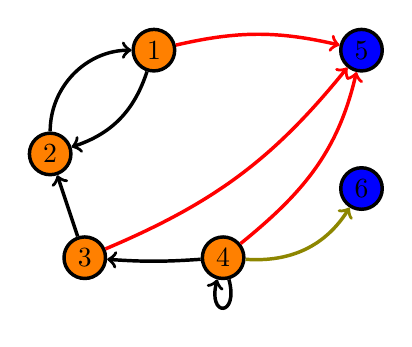
\begin{tikzpicture}
[every node/.style={inner sep=0pt}]
\node (1) [circle, minimum size=15.0pt, fill=orange, line width=1.25pt, draw=black] at (62.5pt, -25.0pt) {\textcolor{black}{1}};
\node (2) [circle, minimum size=15.0pt, fill=orange, line width=1.25pt, draw=black] at (25.0pt, -62.5pt) {\textcolor{black}{2}};
\node (3) [circle, minimum size=15.0pt, fill=orange, line width=1.25pt, draw=black] at (37.5pt, -100.0pt) {\textcolor{black}{3}};
\node (4) [circle, minimum size=15.0pt, fill=orange, line width=1.25pt, draw=black] at (87.5pt, -100.0pt) {\textcolor{black}{4}};
\node (5) [circle, minimum size=15.0pt, fill=blue, line width=1.25pt, draw=black] at (137.5pt, -25.0pt) {\textcolor{black}{5}};
\node (6) [circle, minimum size=15.0pt, fill=blue, line width=1.25pt, draw=black] at (137.5pt, -75.0pt) {\textcolor{black}{6}};
\draw [line width=1.25, ->, color=black] (2) to  [in=180, out=90] (1);
\draw [line width=1.25, ->, color=black] (1) to  [in=18, out=252] (2);
\draw [line width=1.25, ->, color=black] (3) to  (2);
\draw [line width=1.25, ->, color=black] (4) to  [in=356, out=184] (3);
\draw [line width=1.25, ->, color=black, loop below] (4) to (4);
\draw [line width=1.25, ->, color=olive] (4) to  [in=238, out=356] (6);
\draw [line width=1.25, ->, color=red] (4) to  [in=257, out=39] (5);
\draw [line width=1.25, ->, color=red] (3) to  [in=231, out=23] (5);
\draw [line width=1.25, ->, color=red] (1) to  [in=167, out=13] (5);
\end{tikzpicture}

\end{document}
